\chapter{Background}

\section{Decision trees}\label{section:decision_trees}

A decision tree is a supervised learning technique, where given a set of inputs $\textbf{X} = X_1,\dots,X_n$ one tries to predict a response or class $Y$ for an unseen input $X_i$. Decision trees can be used for both classification and regression tasks. In a classification task, $Y$ is a class (also called a label): it is \textit{categorical} (or \textit{discrete}). Consider for instance a set of inputs \textbf{X} where each instance $X_i$ ($i \in [1,n]$) describes the size and the colour of a fruit. For each instance, the associated class in $\textbf{Y}$ could be the type of fruit. A decision tree that is fit on this dataset will learn how to characterise a new, unseen fruit $X_{new}$. In such a scenario, the classification task will therefore be to predict if $X_{new}$ is, say, an apple or an orange. On the other hand, in a regression task, $Y$ is a quantity, a number: it is \textit{numerical} (or \textit{continous}). If our instances in $\textbf{X}$ were now to describe the type and the weight of the fruit, with associated class their size in centimetres, then the regression task would be to predict a real number for the size of $X_{new}$. Figure ~\ref{fig:decision_tree} shows a simple decision tree for both classification and regression.

\begin{figure}[h!]
	\center
  \begin{subfigure}{\linewidth}
  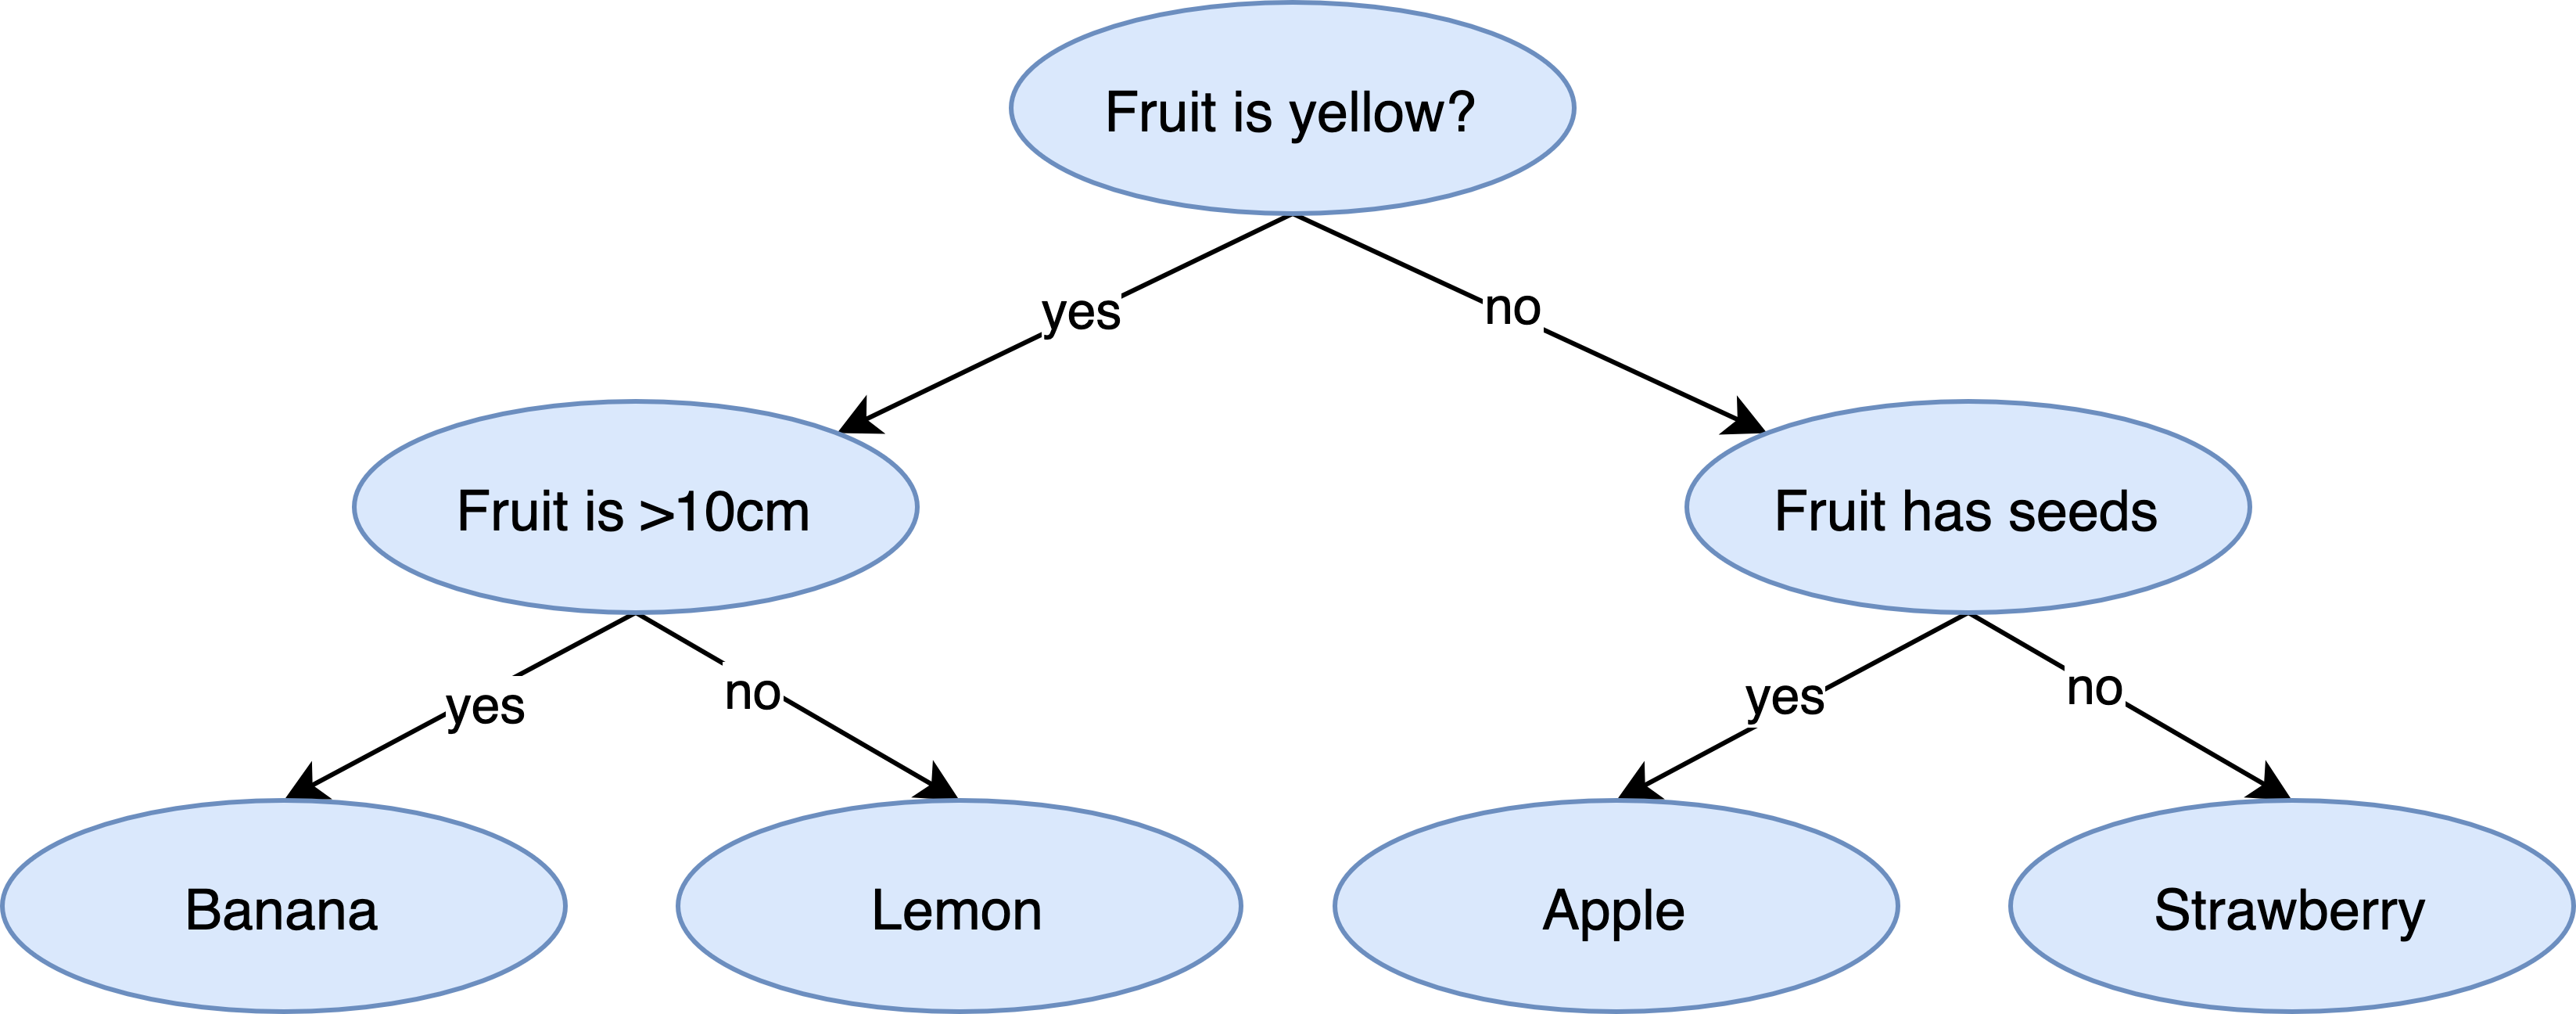
\includegraphics[width=.48\linewidth]{images/background/decision_tree_classification.png}\hfill
  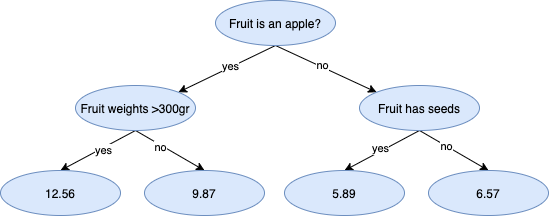
\includegraphics[width=.48\linewidth]{images/background/decision_tree_regression.png}
  \end{subfigure}
  \caption{\label{fig:decision_tree}A classification tree (left) and a regression tree (right).}
\end{figure}


Decision trees consist of:

\begin{itemize}
	\item Nodes: a node represents a decision (or split) to be made about its instances $X_i,\dots,X_j$, where $i, j \in [1,n]$ and $i < j$. This split happens on an attribute and attribute's value of an instance. In the rightmost decision tree in Figure ~\ref{fig:decision_tree}, one such split is on attribute \textit{type of fruit} and attribute's value \textit{apple}.
	\item Edges: an edge corresponds to the outcome of the node's decision, and connects to the next node.
	\item Leaf nodes: a leaf node is a node that is terminal, i.e. it has no children. Leaf nodes hold the prediction results.
\end{itemize}

To classify a new, unseen instance, one simply follows the tree edges until it reaches a leaf node. Constructing a decision tree usually involves a recursive algorithm, such as ID3 \cite{quinlan}. In ID3, the tree construction starts from the root node, and progresses towards the leaf nodes until a maximum depth is reached, controlling how many recursions the algorithm will run through. At each node, the splitting point (i.e., the attribute and attribute's value on which to separate the node's instances) is chosen using the \textit{information gain}.

\begin{definition}[Information Gain \cite{sulq}]
	Let $\textbf{X} = X_1, \dots, X_n$ be a set of inputs (training instances), where each $X_i$ is of the form $(\textbf{x}, y) = (x_1, \dots,x_n,y)$. $x_j$ is the value of the $j^{th}$ attribute of $\textbf{x}$, and $y$ is its corresponding label. The information gain for an attribute $j$ is given by:
	$$IG(\textbf{X}, j) = H(\textbf{X}) - H(\textbf{X}|j)$$
	
	Where $H(\cdot)$ is the Shannon entropy. In other words, the information gain is the difference in entropy before and after the potential split on attribute $j$. Note that after the split, both entropies of resulting nodes are taken into account and added together.
\end{definition}

We can use this measure to rank attributes and choose the best splitting point. While decision trees are rather simple to understand, they come with their fair share of drawbacks:

\begin{itemize}
	\item Prone to overfitting (the trees fit perfectly the training samples but fail to accurately predict unseen samples).
	\item Highly complex when there are many class labels / depth is large.
	\item Low bias and high variance (trees make no assumptions about the target variables, however a change in the training dataset may result in a completely different tree structure).
\end{itemize}

To address the above limitations, one can train multiple trees. In this case, we talk about \textit{ensemble methods}. The idea behind ensemble methods is to combine multiple \textit{weak learners} to form a \textit{strong learner}. Here, a weak learner is a single decision tree and a strong learner is an ensemble of decision trees. The most common ensemble methods are \textit{bagging} and \textit{boosting}. In bagging, one trains several trees on different subsets of the data. As a result, the trees have a different structure and therefore offer different predictions. These trees can be trained in parallel, as they are independent from one another. The final predictions can be computed as the average of all predictions of each individual decision tree. A popular extension of bagging is a \textit{Random Forest} model, where the subsets of data and the trees splitting points are chosen at random.

In boosting, the trees are fitted sequentially, meaning that for an ensemble of $n$ trees, tree $t$ depends on tree $t-1$ for all $t \in [1, n]$. In particular, tree $t$ fits the residual of tree $t-1$. This iterative process is repeated $n$ times, for all trees. Each tree's output ($h(x)$) is usually given a weight $w$ relative to its accuracy. The final predictions are computed as the weighted sum of each tree: $\hat{y}(x) = \sum_t w_t h_t(\textbf{x})$ \cite{woodruff}.  The more often an instance is misclassified, the more important it becomes for the training of the subsequent tree. Training the trees therefore becomes a minimisation problem on the objective function $O(\textbf{x}) = \sum_i l(\hat{y}_i, y_i) + \sum_t \Omega(f_t)$ \cite{xgboost} where $l(\hat{y_i}, y_i)$ is the loss function (i.e. the distance between the truth and the prediction of the $i^{th}$ sample) and $\Omega(f_t)$ is the regularisation function (it penalises the complexity of the $t^{th}$ tree). When the objective function is minimised using \textit{gradient descent}, we talk about \textit{gradient boosting}, which we introduce in the next section.

\section{Gradient boosted decision trees (GBDT)}

Given a convex loss function $l$ and a dataset with $n$ instances $\textbf{X} = X_1,\dots,X_n$, $X_i = (\textbf{x}, y) = (x_1, \dots,x_d, y) \; \forall i \in [1,n]$, GBDT minimises the following objective function at the $t^{th}$ iteration \cite{gbdt_high_dim}:

\begin{equation}\label{eq:gbdt_obj}
	O(\textbf{x})^{(t)} = \sum_i^n \left( g_i f_t (\textbf{x}_i) + \frac{1}{2} h_i f_t^2 (\textbf{x}_i) \right) + \Omega(f_t)
\end{equation}

where $g_i = \partial_{\hat{y}^{(t-1)}}l(y_i, \hat{y}^{(t-1)})$ is the first order gradient statistics of the loss function, $f_t$ is the decision tree at iteration $t$, and $\Omega(f_t) = \frac{1}{2} \lambda \norm{V}^2$ is the regularisation term ($V$ is the leaf weight, $\lambda$ is the regularisation parameter). The tree is built from the root until maximum depth is reached. Assume that $I_L$ and $I_R$ are the instances in the left and right nodes after a split. We have $I = I_L \cup I_R$, and the gain after the split is given by: \cite{xgboost}

\begin{equation}\label{eq:gbdt_gain_full}
	G(I_L, I_R) = \frac{1}{2} \left( \frac{(\sum_{i \in I_L}g_i)^2}{\sum_{i \in I_L} h_i + \lambda} + \frac{(\sum_{i \in I_R}g_i)^2}{\sum_{i \in I_R} h_i + \lambda} - \frac{(\sum_{i \in I}g_i)^2}{\sum_{i \in I} h_i + \lambda} \right)
\end{equation}

For the square loss function, $h_i = 1$ in Equations ~\ref{eq:gbdt_obj} and ~\ref{eq:gbdt_gain_full}. Furthermore, since the last term in the above equation does not depend on the splitting point, and assuming the square loss function is used, Equation~\ref{eq:gbdt_gain_full} can be further simplified to: \cite{dpgbdt}

\begin{equation}\label{eq:gbdt_gain_simplified}
	G(I_L, I_R) = \frac{(\sum_{i \in I_L}g_i)^2}{|I_L| + \lambda} + \frac{(\sum_{i \in I_R}g_i)^2}{|I_R| + \lambda}
\end{equation}

GBDT traverses all combinations of features and features' values to find the best split. If a node has a negative gain or if it is at the maximum depth, then it becomes a leaf node and it is assigned the optimal leaf value:

\begin{equation}\label{eq:gbdt_leaf_value}
	V(I) = - \eta \frac{\sum_{i \in I}g_i}{|I| + \lambda}	
\end{equation}
 
 where $\eta$ is the learning rate, which controls the influence of a single tree. Algorithm ~\ref{algo:gbdt} describes the training process of gradient boosted decision trees.

\begin{algorithm}
	\DontPrintSemicolon
	\SetKwComment{Comment}{$\triangleright$\ }{}
	\SetCommentSty{itshape}
	\caption{GBDTs training process}\label{algo:gbdt}
	\KwIn{$\textbf{X} = X_1,\dots,X_n$: instances, $\textbf{y} = y_1, \dots, y_n$: labels}
	\KwIn{$\lambda$: regularisation parameter, $d_{max}$: maximum depth, $\eta$: learning rate}
	\KwIn{$T$: total number of trees, $l$: loss function}
	\KwOut{An ensemble of trained decision trees.}
	\For{$t=1$ \textbf{to} $T$}{
		Update gradients of all training instances on loss $l$ \;
		\For{d = 1 \textbf{to} $d_{max}$}{
			\For{\textit{each node in current depth}}{
				\For{\textit{each split value i}}{
					$G_i \gets \frac{(\sum_{i \in I_L}g_i)^2}{|I_L| + \lambda} + \frac{(\sum_{i \in I_R}g_i)^2}{|I_R| + \lambda}$ \Comment*[r]{\textcolor{blue}{Equation ~\ref{eq:gbdt_gain_simplified}}}
				}
				Split node on split value $i = \arg\max_i(G_i)$
			}
		}
		\For{\textit{each leaf node i}}{
			$V_i \gets - \eta \frac{\sum_{i \in I}g_i}{|I| + \lambda}$ \Comment*[r]{\textcolor{blue}{Equation ~\ref{eq:gbdt_leaf_value}}}
		}
	}
\end{algorithm}


\section{Differential privacy}\label{sec:dp}

In some cases, the privacy of the individuals that constitute a dataset needs to be preserved. There are several ways to do that, such as $K$\textit{-anonymity}. In $K$-anonymity, the attributes of the individuals are generalised such that a single individual becomes indistinguishable from at least $K-1$ other individuals. Unfortunately, achieving optimal $K$-anonymity is NP-hard and there has been criticism about possible re-identification of the individuals \cite{k-anon}, in particular when the attacker acquires background information about the training data. 

A different approach is to use \textit{differential privacy}. Differential privacy is a mathematical definition that provides provable privacy guarantees \cite{dwork}. It assumes that a potential attacker has almost full knowledge about the training data, and is only uncertain about a single training data point. By leveraging differential privacy, a defender can deny the presence of each and every data point in the training data.

\begin{definition}[$\epsilon$-Differential Privacy \cite{dpgbdt}]
	Let $\epsilon$ be a positive real number and $f$ be a randomised function. The function $f$ is said to provide $\epsilon$-differential privacy if, for any two datasets D and D' that differ by a single record and any output O of function $f$:
	\begin{equation}
		Pr[f(D) \in O] \leq e^{\epsilon} \cdot Pr[f(D') \in O]
	\end{equation}	
\end{definition}

In the above definition, $\epsilon$ is called the \textit{privacy budget}. Intuitively, this budget measures how much privacy the function $f$ offers. The lower this budget, the higher privacy $f$ achieves, i.e. the more a defender can deny the presence of single data points in the training data. To achieve $\epsilon$-differential privacy in practice, the Laplace mechanism and the exponential mechanism are usually adopted \cite{dwork_roth}. The process involves adding noise that is calibrated to the \textit{sensitivity} of $f$.

\begin{definition}[Sensitivity \cite{dpgbdt}]\label{def:sensitivity}
	Let $f: \mathcal{D} \rightarrow \mathcal{R}^d$ be a function. The sensitivity of $f$ is:
	
	\begin{equation}
		\Delta f = \max_{D,D' \in \mathcal{D}} \norm{f(D)-f(D')}_1
	\end{equation}

	where D and D' have at most one different record.
	 
\end{definition}

The sensitivity of $f$ captures the magnitude by which a single datapoint in $\mathcal{D}$ can change the function $f$ in the worst case. In other words, it is a measure of the randomness that we must introduce in order to hide the participation of a single datapoint (to preserve the datapoint's privacy). The $\epsilon$-deniability that a defender gets can fail with probability at most $\Delta f$. Usually, this randomness is drawn from a Laplace distribution.

\begin{definition}[Laplace Distribution]\label{def:laplace_distribution}
	A random variable has a $Lap(\mu, b)$ distribution if its probability density function is:
	
	\begin{equation}
		f(x | \mu, b) = \frac{1}{2b}\exp\left(- \frac{|x-\mu|}{b}\right)
	\end{equation}

	Where $\mu$ is the mean and b is the scale of the distribution.
	
\end{definition}

Combining the previous definitions, we can formally describe the Laplace mechanism and the exponential mechanism.


\begin{theorem}[Laplace Mechanism \cite{dpgbdt}]\label{theorem:lap}
	Let $f: \mathcal{D} \rightarrow \mathcal{R}^d$ be a function. The Laplace mechanism $F$ is defined as:
	
	\begin{equation}
		F(D) = f(D) + Lap(0, \Delta f/\epsilon)
	\end{equation}
	
	Where the noise $Lap(0, \Delta f/\epsilon)$ is drawn from a Laplace distribution with mean $\mu = 0$ and scale $b = \Delta f / \epsilon$. Then $F$ provides $\epsilon$-differential privacy.
	
\end{theorem}

\begin{theorem}[Exponential Mechanism \cite{dpgbdt}]\label{theorem:exp}
	Let $u: (\mathcal{D \times \mathcal{R}}) \rightarrow \R$ be a utility function, with sensitivity $\Delta u$. The exponential mechanism $F$ is defined as:
	
	\begin{equation}
		F(D, u) = \text{choose r} \in \mathcal{R} \; \text{with probability} \propto \; \exp\left(\frac{\epsilon u(D, r)}{2\Delta u}\right)
	\end{equation}
	
	Then $F$ provides $\epsilon$-differential privacy.
	 
\end{theorem}

Theorems ~\ref{theorem:lap} and ~\ref{theorem:exp} provide privacy guarantees for a single function. When using multiple functions, much like in an algorithm, there are considerations to take into account around the privacy budget $\epsilon$. This is considered through two additional theorems: \textit{sequential} composition theorem and \textit{parallel} composition theorem (\cite{dwork_roth}, \cite{dpgbdt}).

\begin{theorem}[Sequential Composition]\label{theorem:sequential_composition}
	Let $f = \{f_1, \dots, f_m\}$ be a series of functions performed sequentially on a dataset. If $f_i$ provides $\epsilon_i$-differential privacy, then $f$ provides $\sum_i^m \epsilon_i$-differential privacy.
\end{theorem}

\begin{theorem}[Parallel Composition]\label{theorem:parallel_composition}
	Let $f = \{f_1, \dots, f_m\}$ be a series of functions performed separately on disjoint subsets of a dataset. If $f_i$ provides $\epsilon_i$-differential privacy, then $f$ provides $\{\max(\epsilon_1,\dots,\epsilon_m)\}$-differential privacy.
\end{theorem}










